As mentioned earlier (see section \ref{sec:intro}) one of the challenges for the agents is to decide when to perform certain actions such as avoidance for the intruder and coverage,pursuits and exploration for the guards. In order to achieve the decision-making process, three different states are created for both guards and the intruder. The three states for the guards are Exploration, Coverage and Catching, and the three states for the intruders are Exploration, Panic and Direct-to-Target. The following diagrams explain the process of state machines of guards and a intruder. 
\begin{figure}
\centering

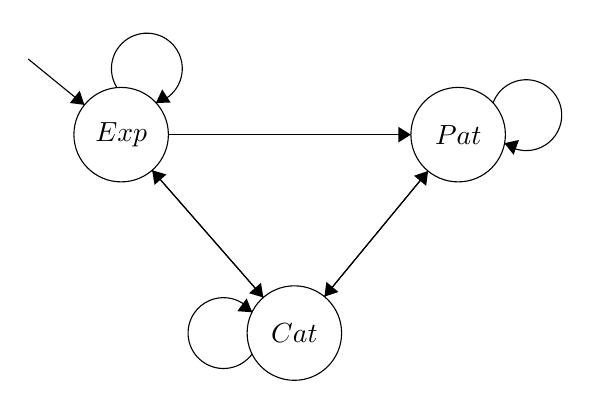
\begin{tikzpicture}[scale=0.2]
\tikzstyle{every node}+=[inner sep=0pt]
\draw [black] (12.3,-7) circle (3);
\draw (12.3,-7) node {$Exp$};
\draw [black] (33.7,-7) circle (3);
\draw (33.7,-7) node {$Pat$};
\draw [black] (23.3,-19.6) circle (3);
\draw (23.3,-19.6) node {$Cat$};
\draw [black] (14.27,-9.26) -- (21.33,-17.34);
\fill [black] (21.33,-17.34) -- (21.18,-16.41) -- (20.42,-17.07);
\draw [black] (21.33,-17.34) -- (14.27,-9.26);
\fill [black] (14.27,-9.26) -- (14.42,-10.19) -- (15.18,-9.53);
\draw [black] (15.3,-7) -- (30.7,-7);
\fill [black] (30.7,-7) -- (29.9,-6.5) -- (29.9,-7.5);
\draw [black] (12.041,-4.023) arc (212.71151:-75.28849:2.25);
\fill [black] (14.51,-4.98) -- (15.45,-4.97) -- (14.91,-4.13);
\draw [black] (35.913,-4.992) arc (159.9454:-128.0546:2.25);
\fill [black] (36.64,-7.54) -- (37.22,-8.28) -- (37.56,-7.34);
\draw [black] (31.79,-9.31) -- (25.21,-17.29);
\fill [black] (25.21,-17.29) -- (26.1,-16.99) -- (25.33,-16.35);
\draw [black] (20.62,-20.923) arc (-36:-324:2.25);
\fill [black] (20.62,-18.28) -- (20.27,-17.4) -- (19.68,-18.21);
\draw [black] (25.21,-17.29) -- (31.79,-9.31);
\fill [black] (31.79,-9.31) -- (30.9,-9.61) -- (31.67,-10.25);
\draw [black] (6.4,-2.2) -- (9.97,-5.11);
\fill [black] (9.97,-5.11) -- (9.67,-4.21) -- (9.04,-4.99);
\end{tikzpicture}

\caption{State machine of the guard. Where $Exp$,$Cov$ and $Cat$ stand for Exploration,Coverage and Catching states respectively.}
\label{fig:my_label}
\end{figure}

\begin{State machine of the guard. Where $Exp$,$DT$ and $Pan$ stand for Exploration, Direct-to-Target and Panic states respectively}
\centering
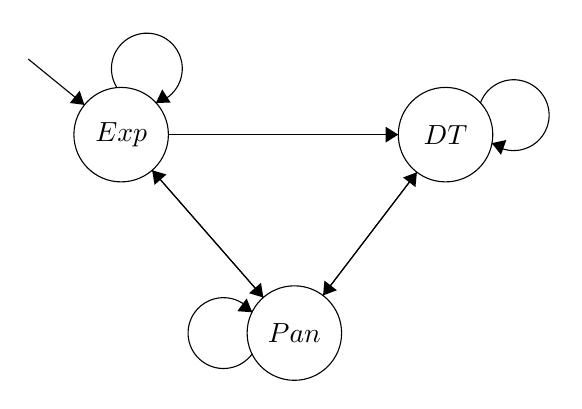
\begin{tikzpicture}[scale=0.2]
\tikzstyle{every node}+=[inner sep=0pt]
\draw [black] (12.3,-7) circle (3);
\draw (12.3,-7) node {$Exp$};
\draw [black] (32.9,-7) circle (3);
\draw (32.9,-7) node {$DT$};
\draw [black] (23.3,-19.6) circle (3);
\draw (23.3,-19.6) node {$Pan$};
\draw [black] (14.27,-9.26) -- (21.33,-17.34);
\fill [black] (21.33,-17.34) -- (21.18,-16.41) -- (20.42,-17.07);
\draw [black] (21.33,-17.34) -- (14.27,-9.26);
\fill [black] (14.27,-9.26) -- (14.42,-10.19) -- (15.18,-9.53);
\draw [black] (15.3,-7) -- (29.9,-7);
\fill [black] (29.9,-7) -- (29.1,-6.5) -- (29.1,-7.5);
\draw [black] (12.041,-4.023) arc (212.71151:-75.28849:2.25);
\fill [black] (14.51,-4.98) -- (15.45,-4.97) -- (14.91,-4.13);
\draw [black] (35.113,-4.992) arc (159.9454:-128.0546:2.25);
\fill [black] (35.84,-7.54) -- (36.42,-8.28) -- (36.76,-7.34);
\draw [black] (31.08,-9.39) -- (25.12,-17.21);
\fill [black] (25.12,-17.21) -- (26,-16.88) -- (25.21,-16.27);
\draw [black] (20.62,-20.923) arc (-36:-324:2.25);
\fill [black] (20.62,-18.28) -- (20.27,-17.4) -- (19.68,-18.21);
\draw [black] (25.12,-17.21) -- (31.08,-9.39);
\fill [black] (31.08,-9.39) -- (30.2,-9.72) -- (30.99,-10.33);
\draw [black] (6.4,-2.2) -- (9.97,-5.11);
\fill [black] (9.97,-5.11) -- (9.67,-4.21) -- (9.04,-4.99);
\end{tikzpicture}
\caption{Caption}
\label{fig:my_label}
\end{figure}

